% Rough analysis of the FC_OpenCourant example results and meshes.
% AI-GENERATED - NOT VERIFIED BY A HUMAN - NO WARRANTY (see the notice and the last section)
% Build: pdflatex ORfe_Example_Analysis.tex (twice)
\documentclass[11pt,a4paper]{article}

\usepackage[utf8]{inputenc}
\usepackage[T1]{fontenc}
\usepackage{lmodern}
\usepackage{microtype}
\usepackage[margin=2.4cm,headheight=14pt]{geometry}
\usepackage{booktabs}
\usepackage{tabularx}
\usepackage{graphicx}
\usepackage{xcolor}
\usepackage{enumitem}
\usepackage{caption}
\usepackage{pgfplots}
\pgfplotsset{compat=1.17}
\usepackage[most]{tcolorbox}
\usepackage{fancyhdr}
\usepackage{lastpage}
\usepackage[firstpage=true]{draftwatermark}
\usepackage[colorlinks=true,linkcolor=blue!50!black,urlcolor=blue!50!black]{hyperref}

\SetWatermarkText{AI-GENERATED -- NOT VERIFIED}
\SetWatermarkScale{0.55}
\SetWatermarkColor[gray]{0.93}

\definecolor{warn}{RGB}{176,40,40}
\pagestyle{fancy}
\fancyhf{}
\fancyhead[L]{\small\textcolor{warn}{\textbf{AI-generated analysis -- not verified by a human -- no warranty}}}
\fancyhead[R]{\small FC\_OpenCourant examples}
\fancyfoot[C]{\small Page \thepage\ of \pageref{LastPage}}
\renewcommand{\headrulewidth}{0.4pt}
\setlist{itemsep=2pt,topsep=4pt}
\emergencystretch=1.5em

\newcommand{\unit}[1]{\,\mathrm{#1}}
\newtcolorbox{notice}[1]{colback=warn!6,colframe=warn,fonttitle=\bfseries,title={#1}}

\title{OpenCourant examples in FreeCAD:\\ a rough analysis of results and meshes}
\author{Generated by an AI assistant (Claude, Anthropic) for the FC\_OpenCourant project}
\date{1 November 2026}

\begin{document}
\maketitle
\thispagestyle{fancy}

\begin{notice}{AI-generated -- not verified by a human}
This document was written by an AI model from automated test runs of the FC\_OpenCourant
workbench (OpenCourant / OpenRadioss in FreeCAD). The numbers were read from solver listings and
result files by scripts, and the interpretations and conclusions are the model's own.
\textbf{No human engineer has checked them.} Do not use them for design, certification or any
decision with safety or financial consequences. The document comes with \textbf{no warranty}
(Section~\ref{sec:warranty}).
\end{notice}

\section{Scope and set-up}

Three example models shipped in \texttt{examples/} were solved and the results compared with
simple reference solutions; the meshes are assessed roughly. A side study compares tetrahedral
meshes with CalculiX.

\begin{itemize}
  \item Software: FreeCAD~1.0.0 (Debian) and 1.1.4 (Flatpak), workbench version 0.0.1,
        OpenCourant \texttt{latest-20261011} (starter commit \texttt{cb760c206e}), Debian~13, x86-64.
  \item Units throughout: mm, t, s, N, MPa. Steel: $E=210\,000\unit{MPa}$, $\nu=0.3$,
        $\rho=7.9\cdot10^{-9}\unit{t/mm^3}$ (Taylor bar: $7.85\cdot10^{-9}$).
  \item Reproduction: the models are rebuilt by \texttt{examples/\allowbreak build\_examples.py}
        (run with \texttt{freecadcmd}), run in the FreeCAD GUI by \texttt{tests/\allowbreak run\_gui\_test.sh},
        and the unit and solver tests by \texttt{tests/\allowbreak tests.py}.
  \item Each case was run once; there is no systematic mesh convergence study.
\end{itemize}

\section{Cantilever beam (FEM workbench, hexahedra)}

\paragraph{Model and mesh.} Beam $100\times10\times10\unit{mm}$, clamped at $x=0$, $F=100\unit{N}$
downwards at the free end, ramped linearly over $10\unit{ms}$. Structured mesh of
$20\times2\times2=40$ eight-node hexahedra (189 nodes), cubes of $5\unit{mm}$ (aspect ratio 1),
\texttt{ELFORM~1} (one integration point, physical hourglass control). No mass scaling.

\paragraph{Numerics.} Time step $0.716\unit{\mu s}$ (estimate from the dilatational wave speed
$\approx 6.0\unit{km/s}$ and $0.9\times5\unit{mm}$: $0.75\unit{\mu s}$), 13\,977 cycles,
$1.6\unit{s}$ wall time. Mass $7.90\cdot10^{-5}\unit{t}$ as expected. At the end the kinetic
energy is $0.05\,\%$ of the internal energy ($9.03\unit{N\,mm}$), so the response is quasi-static;
the external work ($9.04\unit{N\,mm}$) matches $F\delta/2=9.3\unit{N\,mm}$ within a few per cent.

\paragraph{Results.} Tip deflection $0.1868\unit{mm}$ against $0.192\unit{mm}$ from beam theory
with shear deformation ($-2.7\,\%$). The largest nodal von Mises stress is $26.9\unit{MPa}$,
while the bending stress at the clamped surface is $\sigma=Fl\,c/I=60\unit{MPa}$. This is expected
for this mesh: with one integration point per element the stress is sampled at the element
centre, $2.5\unit{mm}$ from the neutral axis and $2.5\unit{mm}$ from the clamp, where beam theory
gives $29\unit{MPa}$; averaging to the nodes lowers it further.

\paragraph{Mesh assessment.} Adequate for the deflection; too coarse for stresses. For surface
stresses use at least 4--8 elements through the thickness or fully integrated elements, and do
not read peak stresses from one-point elements next to a clamp.

\begin{figure}[ht]
\centering
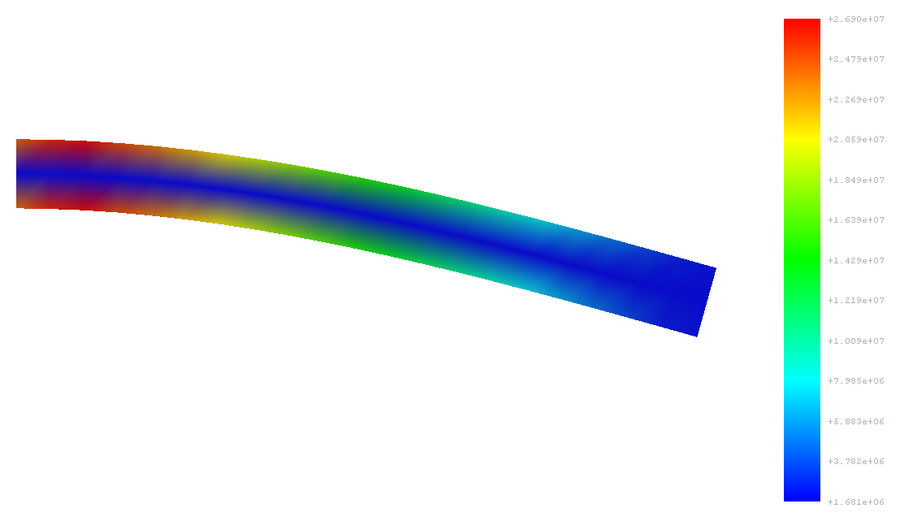
\includegraphics[width=0.62\linewidth]{images/cantilever_beam.png}
\caption{Cantilever, von Mises stress (SI units, Pa) on the deformed shape ($\times100$).}
\end{figure}

\section{Square plate under sudden pressure (FEM workbench, shells)}

\paragraph{Model and mesh.} Plate $200\times200\unit{mm}$, thickness $2\unit{mm}$, all edges
clamped, $q=0.01\unit{MPa}$ applied at $t=0$ and held (\emph{Constant} load curve), no damping.
$20\times20=400$ four-node shells (441 nodes), $10\unit{mm}$ squares, Belytschko--Tsay
(\texttt{ELFORM~2}); span/thickness 100, so a thin plate.

\paragraph{Numerics.} Time step $1.54\unit{\mu s}$, 6\,502 cycles, $0.8\unit{s}$ wall time,
mass $6.32\cdot10^{-4}\unit{t}$ as expected, energy error $\approx0\,\%$.

\paragraph{References.} Static centre deflection of a clamped square plate
$w=0.00126\,q a^4/D=0.131\unit{mm}$ with $D=Et^3/(12(1-\nu^2))$. A load applied suddenly to an
undamped system makes it oscillate between 0 and twice the static value. Fundamental frequency
$f=35.99/(2\pi a^2)\sqrt{D/(\rho t)}\approx447\unit{Hz}$, i.e.\ a period of $2.24\unit{ms}$.

\paragraph{Results.} The centre deflection (Figure~\ref{fig:plate}) oscillates between nearly 0
($0.002$--$0.011\unit{mm}$) and $0.259$--$0.273\unit{mm}$ (twice the static value is $0.262$). The
period between peaks is $2.2\unit{ms}$, and the average over the run is $0.134\unit{mm}$ (static
theory $0.131$, $+2\,\%$). All three agree with the references within a few per cent.

\begin{figure}[ht]
\centering
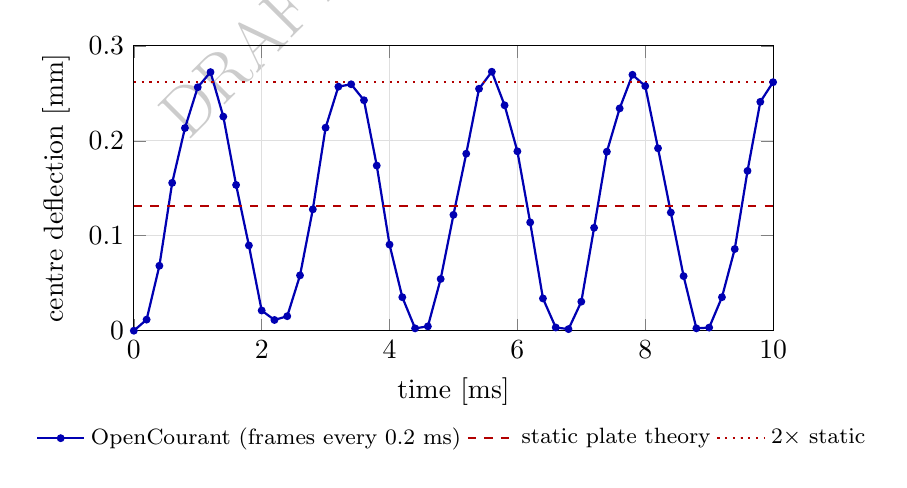
\begin{tikzpicture}
\begin{axis}[width=0.8\linewidth,height=5.2cm,xlabel={time [ms]},ylabel={centre deflection [mm]},
             xmin=0,xmax=10,ymin=0,ymax=0.3,grid=major,grid style={gray!25},
             legend style={font=\footnotesize,at={(0.5,-0.3)},anchor=north,legend columns=3,draw=none}]
\addplot[blue!70!black,thick,mark=*,mark size=1pt] coordinates {
(0.0,0.0000) (0.2,0.0117) (0.4,0.0684) (0.6,0.1557) (0.8,0.2134) (1.0,0.2564) (1.2,0.2723)
(1.4,0.2255) (1.6,0.1535) (1.8,0.0898) (2.0,0.0213) (2.2,0.0113) (2.4,0.0153) (2.6,0.0583)
(2.8,0.1278) (3.0,0.2138) (3.2,0.2570) (3.4,0.2595) (3.6,0.2427) (3.8,0.1739) (4.0,0.0907)
(4.2,0.0353) (4.4,0.0025) (4.6,0.0046) (4.8,0.0545) (5.0,0.1220) (5.2,0.1864) (5.4,0.2548)
(5.6,0.2727) (5.8,0.2374) (6.0,0.1889) (6.2,0.1141) (6.4,0.0340) (6.6,0.0034) (6.8,0.0017)
(7.0,0.0306) (7.2,0.1084) (7.4,0.1885) (7.6,0.2341) (7.8,0.2695) (8.0,0.2576) (8.2,0.1921)
(8.4,0.1245) (8.6,0.0575) (8.8,0.0025) (9.0,0.0033) (9.2,0.0353) (9.4,0.0860) (9.6,0.1683)
(9.8,0.2410) (10.0,0.2617)};
\addlegendentry{OpenCourant (frames every 0.2 ms)}
\addplot[red!70!black,dashed,thick] coordinates {(0,0.131) (10,0.131)};
\addlegendentry{static plate theory}
\addplot[red!70!black,dotted,thick] coordinates {(0,0.262) (10,0.262)};
\addlegendentry{$2\times$ static}
\end{axis}
\end{tikzpicture}
\caption{Plate centre deflection after the sudden pressure load.}
\label{fig:plate}
\end{figure}

\paragraph{Mesh assessment.} Sufficient for the first mode and the centre deflection. The frames
are written every $0.2\unit{ms}$ (about 11 per period), so the extremes are resolved only to about
$\pm3\,\%$; write more frames to measure peaks more precisely. Real plates are damped, so the
undamped oscillation persists longer than it would in a test.

\begin{figure}[ht]
\centering
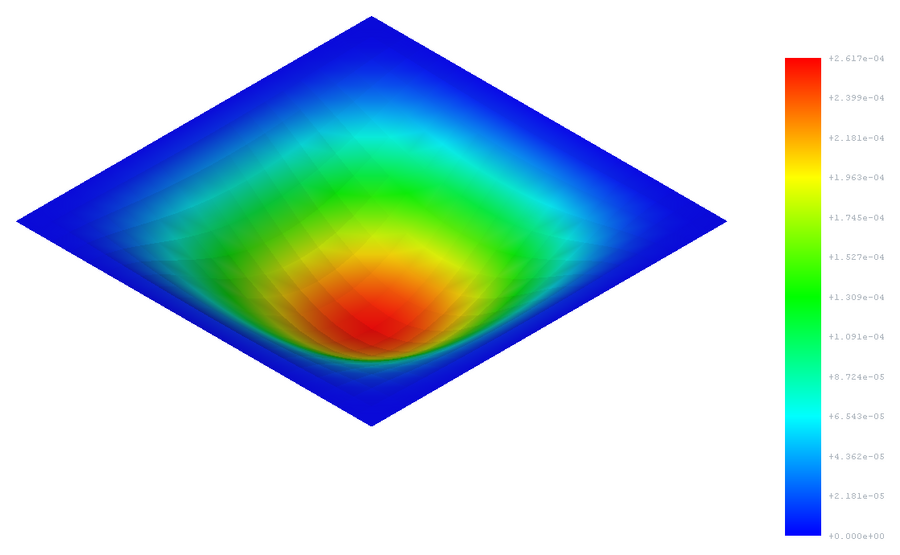
\includegraphics[width=0.55\linewidth]{images/plate_sudden_pressure.png}
\caption{Plate at $10\unit{ms}$, displacement magnitude (m), deformation $\times200$.}
\end{figure}

\section{Taylor impact (keyword deck)}

\paragraph{Model and mesh.} Steel bar $10\times10\times40\unit{mm}$ hitting a rigid wall
(\texttt{*RIGIDWALL\_PLANAR}) at $v=200\unit{m/s}$, bilinear plasticity
(\texttt{*MAT\_PLASTIC\_KINEMATIC}: yield $400\unit{MPa}$, tangent modulus $1000\unit{MPa}$), end
time $60\unit{\mu s}$. $4\times4\times16=256$ hexahedra (425 nodes), cubes of $2.5\unit{mm}$,
\texttt{ELFORM~1}.

\paragraph{Numerics.} The time step drops from $0.158$ to $0.152\unit{\mu s}$ as the elements at
the impact end are compressed; 353 cycles, $0.1\unit{s}$ wall time; mass
$3.14\cdot10^{-5}\unit{t}$ as expected. Initial kinetic energy $\tfrac12 m v^2=6.28\cdot10^{5}\unit{N\,mm}$.
At $52\unit{\mu s}$ the internal energy is $5.84\cdot10^{5}$ and the kinetic energy $2.2\cdot10^{4}$
($3.6\,\%$ of the initial value), so the bar has almost stopped. Internal plus kinetic energy is
$3.4\,\%$ below the initial kinetic energy. A plausible explanation, not checked: the rigid wall
stops the nodes of the impact face instantly; they carry about $1/32$ ($3.1\,\%$) of the mass,
and their kinetic energy is removed.

\paragraph{Results.} The bar shortens from 40.0 to $32.2\unit{mm}$ ($L_1/L_0=0.805$). The
impact end widens from 10.0 to $14.6\unit{mm}$, and the equivalent plastic strain reaches 0.81 at
the impact face. A rough consistency check is Taylor's (1948) formula
$\sigma_y\approx\rho v^2 (L_0-X)/\bigl(2(L_0-L_1)\ln(L_0/X)\bigr)$. With the undeformed length
$X=7.5\unit{mm}$ taken from the simulation (the top part with plastic strain below 0.002) it gives
$\sigma_y\approx390\unit{MPa}$, close to the $400\unit{MPa}$ in the deck. Taylor's formula assumes
rigid--perfectly plastic behaviour, so this checks plausibility only.

\paragraph{Mesh assessment.} Four elements across are coarse for a Taylor test: the mushroom and
the strain gradient at the impact face are spread over one or two elements. In the last frame the
largest element aspect ratio is 3.7 (median 1.5), and impact-face elements are compressed from
2.5 to $1.1\unit{mm}$ edge length. No element inverted, and the run terminated normally. For
quantitative work refine to 8--12 elements across and check the hourglass energy of the
one-point elements, which was not evaluated here.

\begin{figure}[ht]
\centering
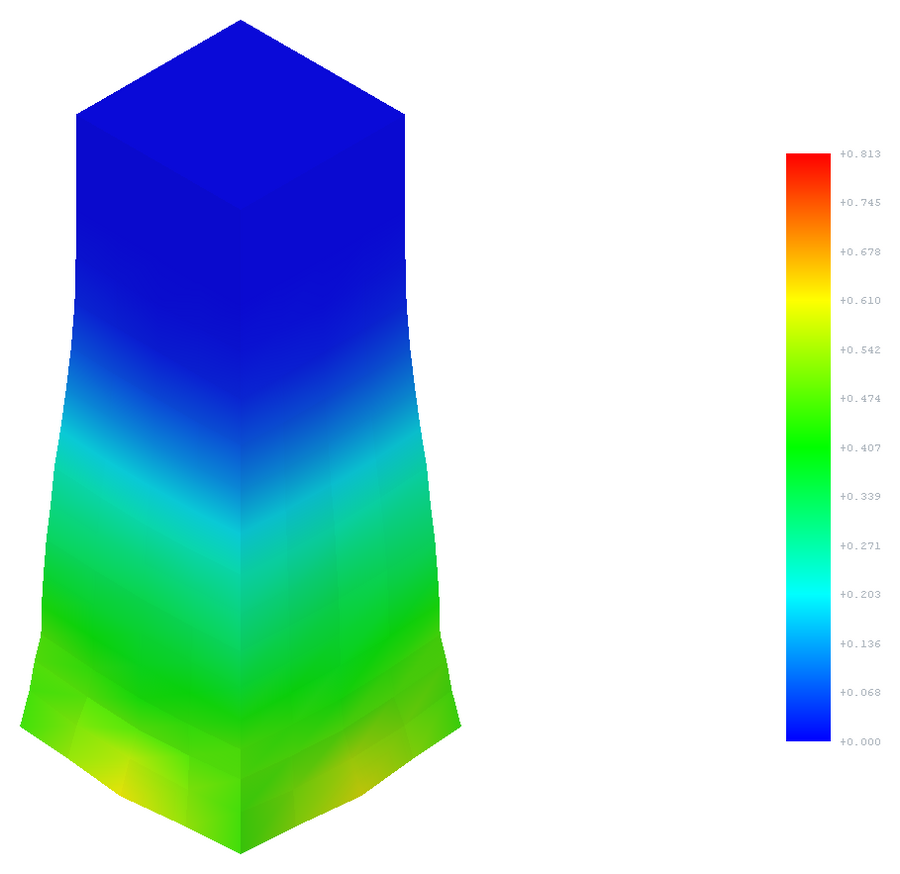
\includegraphics[width=0.42\linewidth]{images/taylor_impact.png}
\caption{Taylor bar at $60\unit{\mu s}$, equivalent plastic strain on the deformed shape (true scale).}
\end{figure}

\section{Side study: tetrahedral meshes of the cantilever}

The same cantilever was meshed with Gmsh and solved with OpenCourant and with CalculiX on the same
mesh settings (Table~\ref{tab:tet}). Linear tetrahedra lock in bending and are too stiff in both
codes, but OpenCourant and CalculiX agree. With 10-node tetrahedra CalculiX matches beam theory
while OpenCourant deflects about $35\,\%$ more, and its starter reports exactly $0.70$ of the
physical mass for every tetra10 mesh tried. The deck's tetra10 node order was checked: every other
midside order is rejected by the starter. This points to the solver's 10-node element (or its
LS-DYNA input mapping) rather than to the translation, but the cause has not been found.

\begin{table}[ht]
\centering\footnotesize
\begin{tabular}{@{}llrrrl@{}}
\toprule
Mesh (Gmsh) & Element & OpenCourant [mm] & CalculiX [mm] & Difference & Note \\
\midrule
$h=4\unit{mm}$ & tetra4  & 0.1329 & 0.1307 & $+1.7\,\%$ & both locked \\
$h=2\unit{mm}$ & tetra4  & 0.1827 & 0.1679 & $+8.8\,\%$ & \\
$h=4\unit{mm}$ & tetra10 & 0.2592 & 0.1908 & $+36\,\%$ & no mass scaling, mass 0.70 \\
$h=2.5\unit{mm}$ & tetra10 & 0.3072 & 0.1910 & $+61\,\%$ & mass scaling: total mass $\times6$ \\
\bottomrule
\end{tabular}
\caption{Tip deflection of the cantilever with tetrahedra; beam theory 0.192\,mm. The last row is
influenced by the large added mass as well.}
\label{tab:tet}
\end{table}

\section{Summary}

\begin{table}[ht]
\centering\small
\begin{tabularx}{\linewidth}{@{}lllX@{}}
\toprule
Case & Quantity & Simulation vs.\ reference & Rough assessment \\
\midrule
Cantilever, hexa8 & tip deflection & $0.187$ vs.\ $0.192\unit{mm}$ ($-2.7\,\%$) & good; stresses need a finer mesh \\
Plate, shells & period & $2.2$ vs.\ $2.24\unit{ms}$ & good \\
 & peak / mean deflection & $0.273$ / $0.134$ vs.\ $0.262$ / $0.131\unit{mm}$ & good (frame spacing limits peaks) \\
Taylor bar & yield from Taylor's formula & $390$ vs.\ $400\unit{MPa}$ & plausible; mesh coarse \\
Cantilever, tetra10 & tip deflection & $0.259$ vs.\ $0.191\unit{mm}$ (CalculiX) & not usable; solver issue open \\
\bottomrule
\end{tabularx}
\end{table}

\section{Limitations of this analysis}

\begin{itemize}
  \item Generated by an AI model and not verified by a human; listing values may have been misread
        and interpretations may be wrong.
  \item One run per case, coarse example meshes, no mesh or time-step convergence study (apart from
        the tetrahedra side study).
  \item The references are simple analytical formulas (beam, plate, Taylor), each with its own
        assumptions; they check plausibility, not correctness.
  \item Hourglass energy, contact and wall forces and strain-rate effects were not evaluated.
  \item Results were read from the last frame or from frames every $0.2\unit{ms}$ and averaged to
        nodes by the workbench, which smooths peaks.
\end{itemize}

\section{No warranty}
\label{sec:warranty}

\begin{notice}{No warranty}
THIS DOCUMENT, THE EXAMPLES AND THE SOFTWARE ARE PROVIDED ``AS IS'', WITHOUT WARRANTY OF ANY KIND,
EXPRESS OR IMPLIED, INCLUDING BUT NOT LIMITED TO THE WARRANTIES OF MERCHANTABILITY, FITNESS FOR A
PARTICULAR PURPOSE, ACCURACY AND NON-INFRINGEMENT. THE ENTIRE RISK AS TO THE QUALITY, ACCURACY
AND USE OF THE RESULTS IS WITH YOU. IN NO EVENT SHALL THE AUTHORS, CONTRIBUTORS OR COPYRIGHT
HOLDERS BE LIABLE FOR ANY CLAIM, DAMAGES OR OTHER LIABILITY ARISING FROM, OUT OF OR IN CONNECTION
WITH THIS DOCUMENT, THE SOFTWARE OR THEIR USE. Simulation results must be verified by a qualified
engineer before they are used for any purpose. The workbench is licensed under the GNU LGPL~2.1 or
later, which contains the same disclaimer; OpenCourant/OpenRadioss is licensed separately under
the AGPL~3.0.
\end{notice}

\end{document}
